\chapter{Modular formalism for stochastic models}
\label{chap:rgspn}

In our current work we aim to propose an approach for the construction of stochastic models from engineering models without human intervention in order to evaluate automatically derived architecture proposals in design-space exploration by stochastic analysis.

The proposed transformation process should be flexible in the sense that---instead of basing our approach on a single engineering modeling language such as \textabbr{UML}~\citep{Rumbaugh04uml}, Sys\mixedabbr{ML}~\citep{Friedenthal16sysml}, \textabbr{AADL}~\citep{Feiler12aadl} or Palladio~\citep{Becker08palladio}---the creation of transformations for new architectural domain-specific languages (\textAbbr{DSL}s) in new problem domains should be supported and should not demand additional specialized knowledge from the users. Therefore the formal models should be based on a stochastic formalism that has sufficient descriptive power to support engineering practice. In addition, compatibility of the derived models with existing stochastic verification tools should be ensured so that recent developments in formal methods may be leveraged for high-performance analysis. Hence reusing an existing formalism is dictated by both \circled{1}~ease of use and \circled{2}~portability.

Analysis tools separate the input formal model and the \emph{query} to be answered \todo*{cite}, which is usually a performance metric to be calculated or a logical requirement to be verified. Therefore, when stochastic models are automatically derived for design-space explaration, \circled{3}~the appropriate queries must also be generated. The queries, which may depend on the structure of the engineering model in the same way as the derived stochastic model, serve as the objective functions and constraints of the exploration strategy.

To achieve these three objectives, in this chapter we turn to stochastic modeling approaches with modules to propose a formalism for the \emph{modules} (or \emph{fragments}) of the stochastic model corresponding to the analyzed aspects of the engineering model. The transformation, which is discussed in \cref{chap:transform}, will instantiate the modules specified by the user to automatically derive the analysis model.

After briefly reviewing related work, we desribe our proposed formalism based on modular Petri nets, an extension of the \textabbr{ISO}/\textabbr{IEC}~15909-1:\citeyear{ISO1590912004} standard on High-level Petri nets with a formally defined module concept~\citep{Kindler09modular}.

In order to \circled{3} generate queries for the stochastic models, we follow \citet{Kindler01modular} and extend modular Petri nets with symbols corresponding to the stochastic properties of interest to encode the queries simultaneously with the structure of the analysis model. Petri nets and their extension to stochastic modeling, generalized stochastic Petri nets (\textAbbr{GSPN}s) are a widely used formalism for the analysis of software and hardware systems~\citep{Murata89petri}. Various tools support \textAbbr{GSPN}s, such as \textabbr{SPNP}~\citep{Hirel00spnp}, \textabbr{SMART}~\citep{Ciardo06smart}, M\"obius~\citep{Courtney09mobius}, Great\mixedabbr{SPN}~\citep{Babar10greatspn} and Petri\-Dot\-Net~\citep{Voros17pdn}. Hence we beleive most of the target audience of our transformation design-space exploration approach are familiar with them. In addition, to aid finding bugs in the analysis models and to contribute to the \circled{1}~ease of use, static typing, which was first proposed for modular high-level Petri nets by \citet{Kindler07modular}, is supported for both the stochastic model and queries. Lastly, models are serialized in the \textabbr{ISO}/\textabbr{IEC}~15909-2:\citeyear{ISO1590922011} \textabbr{PNML} format for \circled{2}~compatibility with a wide variety of external tools.

\section{Related work: Modular stochastic modeling}

In this section we briefly review some existing approaches for modular construction of logical and stochastic formal models, as well as for the specification of properties and metrics of interest over such models. For an overview on performance evaluation techniques for particular component-based software engineering languages, contrasting with our present work that aims to be generic in the engineering \textabbr{DSL}, we direct the interested reader to the survey by~\citet{Koziolek10review}.

We are especially interested in \emph{modular} formalisms that allow assembling structured models from modules (or fragments). While arbitrary combination of modules leads to high expressivity, it also restricts the opportunities for \emph{compositional} verification. On the other hand, a formalism is compositional if the properties of model can be verified recursively by verifying simpler properties of its constituent components. These models are often constructed using \emph{composition operators} that restrict arbitrary modularity in order to enforce property preservation. \todo{Cite!}

We opt for modularity instead of compositionality to avoid restricting the model transformations that will automatically assemble the stochastic models according to an architectural \textabbr{DSL} instance. However, this means solution techniques will have to consider the assembled model in its entierty and cannot depend on preservation of the properties of the components.

\subsection{Modeling formalisms}

Continuous-time Markov chains (\textAbbr{CTMC}s) are common tools for the reliability and performability prediction of critical systems~(see e.g.~\cite{Reibman89markov}). However, instead of modeling with \textAbbr{CTMC}s directly, usually higher-level formalisms are used to obtain more compact models. The semantics of these models are defined in terms of \textAbbr{CTMC}s or related stochastic processes, such as Markov regenerative processes~\citep{Logothetis95mrm,Telek96mrm}. Usually the higher-level formalism belong to one of the following three classes:
\begin{itemize}
\item \textbf{Queueing networks} (\textAbbr{QN}s) describe the routing of \emph{customers} or \emph{work items} between \emph{queues}. The times spent in queues are described by random variables. \todo*{Cite?}
\item \textbf{Stochastic Petri nets} (\textAbbr{SPN}s) are Petri nets where transitions are equiped with expontentially distributed \emph{firing delays}. Generalized stochastic Petri nets (\textAbbr{GSPN}s), may contain transitions with either exponentially distributed delays and \emph{immediate} firing~\citep{Marsan84gspn}. Moreover, deterministic~\citep{Logothetis95mrm} and phase-type distributed~\citep{Longo13phasetype} delays may also be incorporated; however, this makes verification significantly more complicated. Another generalization is the stochastic activity network formalism, where arbitrary input and output gates are allowed~\citep{Sanders01san}.
\item \textbf{Stochastic process algebras} incorporate random timings into the denotational semantics of process calculi~\citep{Hermanns02algebra} while allowing compositional verification. However, composition is syntactically restricted to set of allowed process operators, such as parallel and sequential composition of two subprocesses. An example formalism of this class is the Performance Enchanced Process Algebra (\textabbr{PEPA}) defined by \citet{Hillston95pepa}.
\end{itemize}

Although all \textAbbr{CTMC}s can be expressed with any of these formalism classes, a singnificant advantage of higher-level models is the ability to expresses complicated behaviors of systems with small models. In this regard, \textAbbr{GSPN}s can express \textAbbr{QN}s without increasing model size~\citep{Vernon86comparison}. Comparison of Petri nets and process algebras is more difficult due to the vastly differing modeling styles~\citep{Donatelli95comparison}. The definable composition operators for Petri nets only conserve a limited set of properties; for a review of these operators, we refer to Chapter~2 of the book by \citet{Hejiao12pppnpa}.

\subsection{Query specifications}

\section{Generalized stochastic Petri net modules}

In this section we propose the specification of modules for \textabbr{GSPN}s simultanously with their reward measures and queries. When doing so, contradictions may arise in assembling the stochastic model from modules concerning the initial markings of places, the timings to transition firings and the definitions of the queries. In addition, care must be taken to avoid \emph{circularity} in the merged models and queries: The structure of the model must not depend on the answers to the queries and the values of the stochastic metrics, as the state space and the \textabbr{CTMC} derived from the model is used to answer the queries. Hence circular dependence of the model on the queries makes analysis impossible.

To address these challenges, we base our approach on modular Petri nets~\citep{Kindler01modular}, which define modules as a collection of \emph{symbols} (also referred to as \emph{nodes}) and the \emph{arcs} between them. Petri net places and transitions are represented as symbols. A symbol may either be \emph{concrete} symbol or a \emph{reference} to another symbol. \emph{Imports} of a module are references that are pointed to \emph{exports} of ther modules when the module is instantiated.

A module may only specify additional information about a concrete symbol, such as the initial marking of a concrete place. Thus there is a master-slave relationship between concrete and reference symbols, which avoids contradictions in assembled models. The specification of timed and immediate firing for transitions will be restricted analogously, similarly to the the definition of measures and queries.

We incorporate three new symbol \emph{kinds} into modular Petri nets to construct modular \textabbr{GSPN}s. In addition, an \emph{expression language} is proposed to specify the values of both the stochastic attributes of the model elements, such as transition firing rates, and the performance measures and queries of interest. Circularity in models is avoided by an adapting strict typing to mark invalid dependences as type errors. This approach was inspired by the work of~\citet{Kindler07modular} on strictly typed colored Petri net modules. We call the resulting formalism with extended symbols, expressions and typing \emph{reference generalized stochastic Petri nets} (\textabbr{RGSPN}).

To simplify presentation the separation of module interfaces and implementations, which enable information hiding for the design of modules, will be not considered. Moreover, the assembly of modules into a complete stochastic model is deferred to \cref{chap:transform}. In the remainder of this chapter will will focus on the structure and semantics of single \textabbr{RGSPN} modules and the \emph{inlining} of \textAbbr{RGSPN}s into \textAbbr{GSPN}s without references, which can be analysed with existing tools. 

\subsection{Symbols and edges}

The \textabbr{RGSPN} formalism contains six symbol \emph{kinds} which comprise \textabbr{RGSPN} modules:
\begin{itemize}
\item \textbf{Places} correspond to Petri net places. The token game of the net changes the markings of the places starting from their defined initial marking. The marking is a nonnegative whole number, i.e.~colored variants of \textAbbr{GSPN}s are not currently supported. When \textAbbr{RGSPN}s are shown as graphs places are displayed as \(\bigcirc\)~circles.
\item \textbf{Transitions} correspond to Petri net transitions. They are equipped with a \emph{firing policy}, which is either \emph{timed} or \emph{immediate}. Timed transitions have a \emph{rate} parameter, which is the rate of the exponentially distributed firing delay. Immediate transitions have a probability \emph{weight} and a \emph{priority} consistently with the net-level specification of immediate transitions in \textAbbr{GSPN}s~\citep{}. Graphically, timed transitions are \(\square\)~rectangles, while immediate transitions are \(\blacksquare\)~filled.
\item \textbf{Variables} are expressions that may refer to the markings of transitions, other variables and parameters of the net. The \emph{type} of the expression determines the context where a reference to a variable may appear in the net. Variables are shown as \(\triangle\)~triangles.
\item \textbf{Parameters} are associated with constant real values and express the dependence of the model on continuous parameters. Parameter nodes are preserved during the inlining of the net into a \textabbr{GSPN} as symbolic placeholders. Hence the external tool that solves the \textabbr{GSPN} to answer the queries may constrUct a parametric \textabbr{CTMC} and apply sensitivity analysis~\todo*{cite} or parameter synthesis~\todo*{cite}. The graphical notation for a parameter symbol is a \(\blacktriangle\)~filled triangle.
\end{itemize}

\begin{figure}
  \centering
  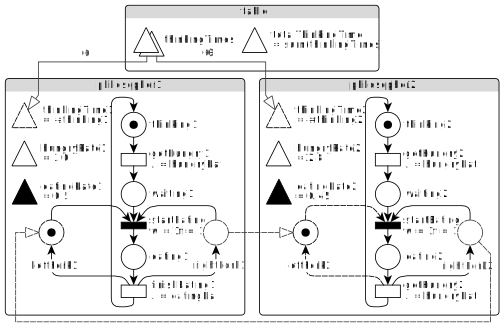
\includegraphics[scale=0.65]{figures/rgspn_example}
  \caption{Example \textabbr{RGSPN} model with two deadlock-free dining philosophers and an aggregate performance measure \textit{totalThinkingTime}.}
\end{figure}

\subsection{Type system}

\subsection{Formal definition}

\section{Expressions}

\section{Inlining of references}

\section{Implementation notes}

\subsection{Reference \textabbr{GSPN} signatures}


Following the terminology of \emph{modular \textabbr{PNML}} models introduced by \citet{Kindler01modular}, we define the signatures of reference \textabbr{GSPN} models as a collection of symbols. Therefore, in our setting places and transitions of Petri nets are different kinds of symbols.

\emph{Variables} are introduced as another kind of symbols to describe the quantitative aspects of the model, including both parameter-dependence and marking-dependence. Parameters that bound from outside, e.g.\ specified in an instance of an engineering model, as well as expressions that are interpreted as marking-dependent random variables can be modeled as variable symbols.

The possible types of symbols are described by the following \textabbr{EBNF}-like grammar:
\begin{equation}
  \begin{aligned}
    \ebnfVar{Type} &\ebnfEq \lit{place} \mid \lit{tran} \mid \ebnfVar{VarType} \mid \bagtype{\ebnfVar{VarType}} \text, \\
    \ebnfVar{VarType} &\ebnfEq \ebnfVar{Dependence}\ \ebnfVar{Pretype} \text,\\
    \rel{Dependence} &\ebnfEq \lit{const} \mid \lit{marking} \mid \lit{analysis}\text, \\
    \ebnfVar{Pretype} &\ebnfEq \lit{int} \mid \lit{double} \mid \lit{boolean} \text.
  \end{aligned} \label{eq:rgspn:type-ebnf}
\end{equation}
The types of \emph{variables}, i.e.~the types \ebnfVar{VarType}, are of the form \(\delta\, \rho\), where \(\delta \in \rel{Dependence}\) and \(\rho \in \rel{Pretype}\). The dependence \(\delta\) describes the aspects of the model that determine the value of the variable.

Variables with \(\lit{const}\) dependence (e.g.~\(\lit{const int}\)) are constant values and may only depend on the structure of the model. In contrast, \(\lit{marking}\) variables are marking-dependent quantities that can be only evaluated and runtime. They can serve as marking-dependent arc inscriptions, transition rates or random variables used in stochastic analyses. Lastly, variables with \(\lit{analysis}\) dependence describe the analyses to be performed of the model.

The pretype \(\rho\) describes the runtime representation of the computed value of the variable. With an abuse of notation, we will write \(\NN\), \(\RR\) and \(\BB\) for the sets of possible values of \lit{int}, \lit{double} and \lit{boolean} variables, respectively.

In addition to variable symbols, \emph{bags} of variables are also introduced to aggregate quantitative aspects defined in multiple parts of the model. An example of such aggregation is the total operational expenses random variable in a performability model, which is the sum of the operational expense random variables of the different system components. The operational expense variables of the individual components can be collected into a bag before summation.

Composition of Petri net modules is aided by \emph{reference} symbols. We will call non-reference symbols \emph{concrete}. Instead of being defined in the Petri net itself, such reference symbols can be connected to other symbols by reference assignments. We follow the conventions in modular \textabbr{PNML}s~\citep{Kindler01modular}, such that reference symbols can refer to a single concrete symbol, while conrete symbols can be assigned to multiple references.

Hence the formal definition of reference \textabbr{GSPN} signatures:

\begin{dfn}
  A \emph{reference \textabbr{GSPN} \paren{\textabbr{RGSPN}} signature} is a tuple \(\Sigma = \ltup S^\Sigma, S_r^\Sigma, \rel{type} \rtup\), where:
  \begin{compactitem}
  \item \(S^\Sigma\) is a set of \emph{symbols}.
  \item \(S_r^\Sigma \subseteq S^\Sigma\) is the set of \emph{reference symbols}.
  \item \(\rel{type}\colon S^\Sigma \to \rel{Type}\) is the \emph{symbol typing function}.
  \end{compactitem}
\end{dfn}

The places, transitions, variables and bags of a signature \(\Sigma = \ltup S^\Sigma, S_r^\Sigma, \rel{type} \rtup\) can be defined as
\begin{align}
  P^\Sigma &= \{s \in S^\Sigma : \rel{type}(s) = \lit{place}\}\text,
  &T^\Sigma &= \{s \in S^\Sigma : \rel{type}(s) = \lit{tran}\}\text, \\
  V^\Sigma &= \{s \in S^\Sigma : \rel{type}(s) \in \rel{VarType}\}\text,
  &B^\Sigma &= \{s \in S^\Sigma : \rel{type}(s) \in \bagtype{\rel{VarType}}\}\text,
\end{align}
respectively. Moreover, the set of all concrete symbols is \(S_c^\Sigma = S^\Sigma \setminus S_r^\Sigma\),
therefore the sets of concrete places \(P^\Sigma_c = P^\Sigma \cap S_c^\Sigma\), transitions \(T^\Sigma_c = T^\Sigma \cap S_c^\Sigma\) and variables \(V^\Sigma_c = V^\Sigma \cap S_c^\Sigma\) can be formed. The superscript \(\Sigma\) will be omitted when the signature is apparent from context.

\subsubsection{Subtyping}

\begin{figure}%
  \begin{tabu}{@{}XX@{}}
    {\begin{tabu}{@{}X[c]r@{}}
        \(\alpha \subtype \alpha\), & \Tagstyle{S-Refl} \\
        \(\lit{const} \subtype \lit{marking}\), & \Tagstyle{SD-Marking} \\
        \(\lit{const} \subtype \lit{analysis}\), & \Tagstyle{SD-Analysis} \\
        \(\lit{int} \subtype \lit{double}\), & \Tagstyle{SPt-Double}
      \end{tabu}}
    & {\begin{tabu}{@{}X[c]r@{}}
        \(\dfrac{
          \delta_1 \subtype \delta_2 \quad \rho_1 \subtype \rho_2
        }{
          \delta_1\,\rho_1 \subtype \delta_2\,\rho_2
        }\), & \Tagstyle{S-Var} \\[1.5ex]
        \(\dfrac{
          \tau_1 \subtype \tau_2
        }{
          \bagtype{\tau_1} \subtype \bagtype{\tau_2}
        }\) & \Tagstyle{S-Bag}
      \end{tabu}}
  \end{tabu}
  \caption{Subtyping rules for \textabbr{RGSPN} signatures.}
  \label{fig:rgspn:subtype}
\end{figure}

In order to capture valid and invalid assignments of references, the set of types defined in \cref{eq:rgspn:type-ebnf} is augmented with a subtyping relation to express compatibility between symbols. The \emph{\textabbr{RGSPN} subtyping relation} is the largest binary relation \({\subtype} \subseteq \rel{Type}^2 \cup \rel{Dependence}^2 \cup \rel{Pretype}^2\) which satisfies the subtyping rules shown in \cref{fig:rgspn:subtype}.

The rules \textsc{S-Relf} ensures that subtyping is reflexive over both types, dependences and types. The compatibility of variable types is captured by \textsc{S-Var} to follow both dependence and pretype subtyping, while \textsc{S-Bag} makes bags covariant in their member types. \textsc{SD-Marking} and \textsc{SD-Analysis} allow the introduction of dependences, i.e.~a constant may be used where a marking dependent value is required, albeit it depends on the current marking in a trivial way. \textsc{SPt-Double} lets \lit{int} values be coerced into \lit{double} values; however, there are no coertions for \lit{boolean}.

We remark that it would be possible to include more elaborate abstract syntax and subtyping rules for types, for example to describe colored Petri nets. In colored nets, \emph{color classes} or \emph{sorts} are associated with places and scalar token counts are replaced by multisets over the elements of the color class. \citet{Kindler07modular} studied modular colored Petri nets with sort and operator symbols. A sort symbol reference is a color class that can be imported into the module from outside and is thus left abstract inside the module. Types of places thus may depend on the sort symbols.

In addition, modular colored nets may also contain \emph{operator} symbols, which transform members of a color class into another. In our type theoretical framework, these can be modeled by \(\ebnfVar{Type} \ebnfEq \ldots \mid \ebnfVar{Type} \to \ebnfVar{Type}\), i.e.~symbols of type \(\tau \to \tau'\) are operators that transform values of type \(\tau\) into values of type \(\tau'\). Polyporphic operators may also be considered. The arising challenges could be handled by tools from simply typed lambda calculus and system F with subtyping (see e.g.~\citet[Chapters~15 and~26]{Pierce02tapl}).

\subsubsection{Symbol assignment}

An \emph{assignment} between of a reference symbol \(r \in S_r\) and another symbol \(s \in S\) signifies that any occurrence of \(r\) should be replaced by \(s\). Similarly, \emph{appending} the sybol \(s\) symbol to a bag \(b \in S\) signifies that any aggregation expression that refers to \(b\) should account for the value of \(s\).

\begin{dfn}
  \label{dfn:rgspn:assign}
  The relation \({\assign} \subseteq S_r \times S\) is an \emph{\textabbr{RGSPN} assignment relation} of the signature \(\Sigma = \ltup S, S_r, \rel{type} \rtup\) subject to the following conditions:
  \begin{compactenum}
  \item \(\rel{type}(s) \subtype \rel{type}(r)\) for all \(r \assign s\). \label{it:rgspn:assign:subtype}
  \item If \(r \assign s_1\) and \(r \assign s_2\) then \(s_1 = s_2\), i.e.~the relation \(\assign\) is the graph of a function. \label{it:rgspn:assign:single}
  \item There are no \emph{reference cycles} of symbols, that is, sequences \(r_1, r_2, \ldots, r_k, r_{k + 1} = r_1\), where \(r_i \assign r_{i + 1}\) for all \(i = 1, 2, \ldots, k\). \label{it:rgspn:assign:cycle}
  \end{compactenum}
  If for each \(r \in S_r\) there exists some \(s \in S\) such that \(r \assign s\), we say that \(\assign\) is \emph{fully specified}.
\end{dfn}

Condition~\ref{it:rgspn:assign:subtype} ensures that type of \(s\) is a subtype of the type of \(r\), thus \(s\) can be used anywhere \(r\) would occur. Condition~\ref{it:rgspn:assign:single} forbids multiple assignments to the same reference, while condition~\ref{it:rgspn:assign:cycle} prevents cycles of references, where the recursive substitution of references with their assigned symbols would fail to terminate.

As assignments between references are permitted, the relation \rel{assign} must be traversed recursively to extract the concrete symbols corresponding to reference. The condition for fully specified assignment relations ensures that no reference symbol is encountered during this traversal which does not have an assigned symbol. 
\begin{dfn}
  The \emph{concretization} of symbols according to an \textabbr{RGSPN} assignment relation \({\assign} \subseteq S_r \times S\) of \(\Sigma = \ltup S, S_r, \rel{type} \rtup\) is \(\rel{conc}\colon S \to S_c\), where
  \begin{equation}
    \rel{conc}(s) = \begin{cases}
      s, & \text{if \(s \in S_c\),} \\
      \rel{conc}(s'), & \text{if \(s \in S_r\) and \(s \assign s'\).}
    \end{cases}
  \end{equation}
  This function is well-defined if \(\assign\) is fully specified.
\end{dfn}

While only a single symbol can be assigned to a reference, a bag may have many members that describe quantitative aspects that are to be aggregated from different parts of the model. Thus a bag symbol may have any number of \emph{member symbols}.
\begin{dfn}
  The multiset relation \({\member} \in \rel{Multiset}(B \times S)\) is an \emph{\textabbr{RGSPN} bag membership relation} of the signature \(\Sigma = \ltup S, S_r, \rel{type} \rtup\) if \(\bagtype{\rel{type}(s)} \subtype \rel{type}(b)\) for all \(b \member s\).
\end{dfn}

Note that while the assignment relation \(\assign\) is a set of pairs, \(\member\) is defined as a multiset of pairs. To illustrate the advantages of multiset semantics, consider the signature \(\ltup \{b, s, r\}, \{r\}, \rel{type} \rtup\) in the following example: Let \(b \in S_c\) be a bag symbol of type \(\bagtype{\tau}\), and let \(s \in S_c\) and \(r \in S_r\) be a concrete and reference symbol of type $\tau$, respectively. Moreover, let the assignment relation be \((\assign) = \{\ltup r, s\rtup\}\) while the bag membership relation is \((\member) = \Lbag \ltup b, s\rtup, \ltup b, r\rtup\Rbag\). The concrete symbol \(s\) appears twice in the bag \(b\), once by a direct membership pair in \(\member\) and once indirectly by being assigned to the reference \(r\). When we replace \(r\) by its concretization \(\rel{conc}(r) = s\), the membership relation becomes \((\member)' = \Lbag \ltup b, s\rtup, \ltup b, s\rtup\Rbag\), hence \(s\) still appears twice. Were set semantics used instead, the multiplicity of \(r\) would have been changed from 2 to 1 in the bag \(b\).

Alternatively, assigning two symbols with equal concretizations to the same bag could be forbidden, making the \(\member\) from the example above an incorrect bag membership relation. We followd the more lenient route by multiset semantics, as it yields more predictable behavior when a union \((\member) = (\member)_1 \uplus (\member)_2\) of membership relations is considered.

\begin{dfn}
  The \emph{member symbols} of bag symbols according to an \textabbr{RGSPN} assignment relation \({\assign} \subseteq S_r \times S\) and bag membership relation \({\member} \in \rel{Multiset}(B \times S)\) of \(\Sigma = \ltup S, S_r, \rel{type} \rtup\) is \(\rel{members}\colon B \to \rel{Multiset}(S_c)\), where
  \begin{equation}
    \label{eq:rgspn:member-symbols}
    \rel{members}(b) = \Lbag \rel{conc}(r) : b' \member r, \rel{conc}(b) = \rel{conc}(b')\Rbag \text.
  \end{equation}
  This function is well-defined if \(\assign\) is fully specified and yields the empty multiset for bags with no member symbols.
\end{dfn}

The process of replacing symbols with their concretizations in the membership relation is captured in the member symbols function to find the members of a bag. \Cref{eq:rgspn:member-symbols} uses concretization to handle the cases when either the bag, its member symbols or both are references. The multiplicities of members are preserved because \(\rel{members}\) is multiset-valued.

\subsubsection{Signature composition}

While the proposed assignment and membership relations are interpreted over a single signature \(\Sigma\), it is possible compose modules by \textabbr{RGSPN} assignment. Let the \emph{disjoint union} \(\Sigma = \Sigma_1 \sqcup \Sigma_2\) of \(\Sigma_1 = \ltup S_1, S_{r,1}, \rel{type}_1 \rtup\) and \(\Sigma_2 = \ltup S_2, S_{r,2}, \rel{type}_2 \rtup\) denote the signature \(\Sigma = \ltup S_1 \sqcup S_2, S_{r,1} \sqcup S_{r,2}, \rel{type} \rtup\) with \(\rel{type}\) extended to \(S_1 \sqcup S_2\) in the straightforward way. This operator is commutative, associative and the the \emph{empty signature} \(\Sigma_\emptyset = \ltup \emptyset, \emptyset, \rel{type}_\emptyset\rtup\) is its unit, where \(\rel{type}_\emptyset\) is trivial.

The \emph{composition} of \textabbr{RGSPN} modules with signatures \(\Sigma_1\) and \(\Sigma_2\) can be described by the assigment relation \((\assign) = (\assign)_1 \cup (\assign)_2 \cup (\assign)_{1,2}\) over the signature \(\Sigma_1 \sqcup \Sigma_2\), where \((\assign)_1\) and \((\assign)_2\) are reference assignments in \(\Sigma_1\) and \(\Sigma_2\), respectively, while \((\assign)_{1,2}\) intermixes the symbols of the two source signatures. The membership relation \((\member) = (\member)_1 \uplus (\member)_2 \uplus (\member)_{1,2}\) factors similarly via multiset union. This construction generalizes to the composition of multiple modules by exploiting associativity and commutativity.

\subsection{Expressions}

In this section we propose an abstract syntax for expressions that describe the quantitative aspects of reference \textabbr{GSPN} models. Such expressions will describe the arc inscription, the initial marking a and the firing distributions of the Petri net. In addition, the reward measures to be evaluated will be also written in the same manner.

Given an \textabbr{RGSPN} signature \(\Sigma\) we define \(\rel{Expr}(\Sigma)\) as the set of valid expressions over \(\Sigma\). This set is described with an \textabbr{EBNF}-like notation as follows. Note that we only consider finite expression trees, thus \(\rel{Expr}(\Sigma)\) is a least fixed point described by the following \textabbr{EBNF}-like grammar:
\begin{equation}
  \label{eq:rgspn:expression}
  \begin{aligned}
    \ebnfV{\rel{Expr}(\Sigma)} &\ebnfEq \ebnfVar{Unary}\; \ebnfV{\rel{Expr}(\Sigma)}
    \mid \ebnfV{\rel{Expr}(\Sigma)} \mathbin{\ebnfVar{Binary}} \ebnfV{\rel{Expr}(\Sigma)} \\*
    &\ebnfCont \lit{if (\ebnfV{\rel{Expr}(\Sigma)}) \ebnfV{\rel{Expr}(\Sigma)} else \ebnfV{\rel{Expr}(\Sigma)}} \\*
    &\ebnfCont \ebnfVar{Aggregate} \lit{(} \ebnfV{B^\Sigma} \lit{)} \mid
      \ebnfV{V^\Sigma} \mid \lit{\#} \ebnfV{P^\Sigma} 
      \mid \ebnfVar{Literal} \text, \\
    \ebnfVar{Unary} &\ebnfEq \lit{+} \mid \lit{-} \mid \lit{!} \text, \\
    \ebnfVar{Binary} &\ebnfEq \lit{+} \mid \lit{-} \mid \lit{*} \mid \lit{/}
    \mid \lit{==} \mid \lit{!=} \mid \lit{<} \mid \lit{<=} \mid \lit{>} \mid \lit{>=}
    \mid \lit{\&\&} \mid \lit{||} \text, \\
    \ebnfVar{Aggregate} &\ebnfEq \lit{sum} \mid \lit{prod}
    \mid \lit{all} \mid \lit{any} \text, \\
    \ebnfVar{Literal} &\ebnfEq \ebnfV{\NN} \mid \ebnfV{\RR} \mid \ebnfV{\BB} \text.
  \end{aligned}
\end{equation}

Elements of \(\rel{Expr}(\Sigma)\) are arithmetic expressions containing basic unary and binary operators, conditionals, literals \lit{int}, \lit{double} and \lit{boolean} values, as well as mentions of the symbols of \(\Sigma\). \(\rel{Expr}(\Sigma)\) contains unary, binary and aggregation operators, as well as conditional expressions; however, the exact set of available operators will not be important in the following discussion. We suppose that the set of available operators is sufficient for expressing the quantitative aspects required by the modeled problem.

Concrete and reference variables \(V^\Sigma\) may be mentioned in expressions as-is and are interpreted as references to the values they hold. In contrast, collection variables must be paired with an \emph{aggregation operator} to turn the multiple variables assigned to them into a single value. Place symbols \(P^\Sigma\) can be also mentioned and correspond to \lit{marking} dependent expressions by referring to the number of tokens on the place.

\subsubsection{Typing}

The relation \(\Sigma \vdash e \oftype \tau\) assigns a type \(\tau\) to an expression \(e \in \rel{Expr}(\Sigma)\) in the context of an \textabbr{RGSPN} signature \(\Sigma\). This typing relation is the largest ternary relation which satisfies the inference rules shown in~\cref{fig:rgspn:typing}. If an expression is assigned a type, its type is always of the form \(\delta\,\rho\).

\begin{figure}
  \begin{tabu}{@{}X[c]r@{}}
    \(\dfrac{{\diamond} \in \{\lit{+}, \lit{-}\}
      \quad \rho \in \{\lit{int}, \lit{double}\}
      \quad \Sigma \vdash e \oftype \delta\,\rho
    }{\Sigma \vdash \mathop{\diamond} e \oftype \delta\,\rho}\),
    & \Tagstyle{T-Unary\(\pm\)} \\[1ex]
    \(\dfrac{\Sigma \vdash e \oftype \delta\,\lit{boolean}
    }{\Sigma \vdash \mathop{\lit{!}} e \oftype \delta\,\lit{boolean}}\),
    & \Tagstyle{T-UnaryNot} \\[1ex]
    \(\dfrac{{\diamond} \in \{\lit{+}, \lit{-}, \lit{*}, \lit{/}\}
      \quad \rho \in \{\lit{int}, \lit{double}\}
      \quad \Sigma \vdash e_1 \oftype \delta\,\rho
      \quad \Sigma \vdash e_2 \oftype \delta\,\rho
    }{\Sigma \vdash e_1 \mathbin{\diamond} e_2 \oftype \delta \,\rho}\),
    & \Tagstyle{T-BinNumeric} \\[1ex]
    \(\dfrac{{\diamond} \in \{\lit{==}, \lit{!=}\}
      \quad \Sigma \vdash e_1 \oftype \delta\,\rho
      \quad \Sigma \vdash e_2 \oftype \delta\,\rho
    }{\Sigma \vdash e_1 \mathbin{\diamond} e_2 \oftype \delta\,\lit{boolean}}\),
    & \Tagstyle{T-BinEq} \\[1ex]
    \(\dfrac{{\diamond} \in \{\lit{<}, \lit{<=}, \lit{>}, \lit{>=}\}
      \quad \Sigma \vdash e_1 \oftype \delta\,\lit{double}
      \quad \Sigma \vdash e_2 \oftype \delta\,\lit{double}
    }{\Sigma \vdash e_1 \mathbin{\diamond} e_2 \oftype \delta\,\lit{boolean}}\),
    & \Tagstyle{T-BinCompare} \\[1ex]
    \(\dfrac{{\diamond} \in \{\lit{\&\&}, \lit{||}\}
      \quad \Sigma \vdash e_1 \oftype \delta\,\lit{boolean}
      \quad \Sigma \vdash e_2 \oftype \delta\,\lit{boolean}
    }{\Sigma \vdash e_1 \mathbin{\diamond} e_2 \oftype \delta\,\lit{boolean}}\),
    & \Tagstyle{T-BinLogical} \\[1ex]
    \(\dfrac{\Sigma \vdash e_1 \oftype \delta\,\lit{boolean}
      \quad \Sigma \vdash e_2 \oftype \delta\,\rho
      \quad \Sigma \vdash e_3 \oftype \delta\,\rho
    }{\Sigma \vdash \lit{if (\(e_1\)) \(e_2\) else \(e_3\)} \oftype \delta\,\rho}\), &
    \Tagstyle{T-If} \\[1ex]
    \(\dfrac{\rel{agg} \in \{\lit{sum}\mkern1mu, \lit{prod}\}
      \quad \rho \in \{\lit{int}, \lit{double}\}
      \quad \rel{type}(b) = \bagtype{\delta\,\rho}
    }{\Sigma \vdash \lit{\rel{agg}(\(b\))} \oftype \delta\,\rho}\),
    & \Tagstyle{T-AggNumeric} \\[1ex]
    \(\dfrac{\rel{agg} \in \{\lit{all}, \lit{any}\}
      \quad \rel{type}(b) = \bagtype{\delta\,\lit{boolean}}
    }{\Sigma \vdash \lit{\rel{agg}(\(b\))} \oftype \delta\,\lit{boolean}}\),
    & \Tagstyle{T-AggLogical} \\[1ex]
    \multicolumn{2}{@{}p{\linewidth}@{}}{
      \begin{tabu}{@{}X[c]rX[c]r@{}}
        \(v \oftype \rel{type}(v)\), & \Tagstyle{T-Var}
        & \(\lit{\#} p \oftype \lit{marking int}\), & \Tagstyle{T-Marking} \\[.5ex]
        \(\dfrac{\ell \in \rel{Literal}_\rho}{\Sigma \vdash \ell \oftype
          \lit{const}\,\rho}\), & \Tagstyle{T-Literal}
        & \(\dfrac{\Sigma \vdash e \oftype \tau\quad \tau \subtype
          \tau'}{\Sigma \vdash e \oftype \tau'}\), & \Tagstyle{T-Sub}
      \end{tabu}
    }
  \end{tabu}
  \bigskip
  where \(\rel{Literal}_{\lit{int}} = \mathbb{N}\),
  \(\rel{Literal}_{\lit{double}} = \mathbb{R}\) and
  \(\rel{Literal}_{\lit{boolean}} = \mathbb{B}\).
  \caption{Typing rules for expressions.}
  \label{fig:rgspn:typing}
\end{figure}

The types of unary operators, binary operators, conditional and aggregate expressions are captured by the rules \textsc{T-Un}, \textsc{T-Bin}, \textsc{T-If} and \textsc{T-Agg}. Instead of introducing polyporphic types for operators and typing rules for operator application, the typing rules for all operators are written out explicitly. While this approach increases the number of typing rules considerably, the lack of function types and polymorphic types allows the syntax of \(\rel{Type}\) to remain simple. If more generality is desired, operator types can be introduced to the syntax of types to support e.g.~user-defined operators. Such types are also used in modular colored Petri nets~\citep{Kindler07modular}.

In spite of being handled only in the type derivation rules, operators are polymorphic in the types of the arguments. All compound expressions are \emph{dependency polymorphic}, that is, the types of their arguments may have any dependency qualifier \(\delta\), which will be inherited by the type of the whole expression. In addition, most operators are also polymorphic in the pretypes of their arguments.

Variable and marking references are handled by \textsc{T-Var} and \textsc{T-Marking}. Referring to markings of places always produces a \lit{marking} dependent \lit{int}. In contrast, \textsc{T-Literal} assigns \lit{const} types to literal constants. Lastly, \textsc{T-Sub} allows the use of subtyping in type derivations.

\subsubsection{Analysis expressions}

The abstract syntax presented in \cref{eq:rgspn:expression} contains no expressions that produce values of dependen \lit{analysis}. In this section we propose a small set of analyses which treat \lit{marking} dependent expressions as random variables,
\begin{equation}
  \begin{aligned}
    \ebnfV{\rel{Expr}(\Sigma)} &\ebnfEq \ldots \\
    &\ebnfCont \lit{transient(\(\ebnfV{\rel{Expr}(\Sigma)}\), \(\ebnfV{\rel{Expr}(\Sigma)}\))} \mid \lit{accumulate(\(\ebnfV{\rel{Expr}(\Sigma)}\), \(\ebnfV{\rel{Expr}(\Sigma)}\))} \\
    &\ebnfCont \lit{steadystate(\(\ebnfV{\rel{Expr}(\Sigma)}\))} \mid \lit{mtff(\(\ebnfV{\rel{Expr}(\Sigma)}\))} \text.
  \end{aligned}
\end{equation}
These expressions enable embedding the analyses to be performed directly into the \textabbr{RGSPN} model.

\begin{figure}
  \begin{tabu}{@{}X[c]r@{}}
    \(\dfrac{\Sigma \vdash e_1 \oftype \lit{marking double}
      \quad \Sigma \vdash e_2 \oftype \lit{const double}
    }{\Sigma \vdash \lit{transient(\(e_1\), \(e_2\))} \oftype \lit{analysis double}}\),
    & \Tagstyle{T-Transient} \\[1ex]
    \(\dfrac{\Sigma \vdash e_1 \oftype \lit{marking double}
      \quad \Sigma \vdash e_2 \oftype \lit{const double}
    }{\Sigma \vdash \lit{accumulate(\(e_1\), \(e_2\))} \oftype \lit{analysis double}}\),
    & \Tagstyle{T-Accumulate} \\[1ex]
    \(\dfrac{\Sigma \vdash e \oftype \lit{marking double}
    }{\Sigma \vdash \lit{steadystate(\(e\))} \oftype \lit{analysis double}}\),
    & \Tagstyle{T-Steadystate} \\[1ex]
    \(\dfrac{\Sigma \vdash e \oftype \lit{marking boolean}
    }{\Sigma \vdash \lit{mtff(\(e\))} \oftype \lit{analysis double}}\),
    & \Tagstyle{T-Mtff}
  \end{tabu}
  \caption{Typing rules for analysis expressions.}
  \label{fig:rgspn:analysis-typing}
\end{figure}

The embedded analysis expressions are explicitly tagged with the \lit{analysis} dependence according to the typing rules in \cref{fig:rgspn:analysis-typing}. Thus analysis results can be forbidden from influencing the behaviour of the Petri net. For example, the steady-state expectation of a random variable cannot influence the timing of a stochastic Petri net transition, because the timing determines the steady-state of the model.

The \lit{transient} and \lit{accumulate} analyses take a random variable of type \lit{marking double} and a time instant of type \lit{const double}. The result of the analysis is the expected value of the random variable and the expected value of the time integral of the random variable at the specified time moment. This value can be determined by transient stochastic analysis of the underlying continuous-time Markov chain (\textabbr{CTMC}) of the stochastic model.

Steady-state analysis is possible by the expression \lit{steadystate}, which also takes a \lit{marking double} random variable and returns its expected value according to the steady-state distribution of the underlying \textabbr{CTMC}.

Mean-time-to-first-failure analysis, also called mean time to reach a state partition, is provided by \lit{mtff}, which takes a \lit{marking boolean} expression and returns the mean time for the expression to become \lit{true}.

\subsection{Reference \textabbr{GSPN} definitions}

In this section we consider generalized stochastic Petri nets over an \textabbr{RGSPN} signatures. These nets may contain reference symbols, such as reference places and transitions, hence the name reference \textabbr{GSPN}.

Similarly to generalized stochastic Petri nets, places are annotated with initial markings, while transitions are annotated with priorities and weights. To describe the quantitative aspects of the model, variable symbols are annotated with algebraic expressions over the net's signature.

\begin{dfn}
  \label{dfn:rgspn:rgspn}
  A \emph{reference \textabbr{gspn}} is a tuple \(\rel{RGSPN} = \ltup \Sigma, F, W, M_0, \pi, \lambda, \rel{value} \rtup\), where:
  \begin{compactitem}
  \item \(\Sigma\) is a reference \textabbr{GSPN} signature.
  \item \(F \subseteq P \times \{\inarc, \outarc, \inharc\} \times T\) is the set of \emph{arcs}.
  \item \(W\colon F \to \rel{Expr}(\Sigma)\) is the \emph{arc inscription function}.
  \item \(M_0\colon P_c \to \rel{Expr}(\Sigma)\) is the \emph{initial marking function}.
  \item \(\pi\colon T_c \to \rel{Expr}(\Sigma) \cup \{\bot\}\) is the \emph{transition priority function}.
  \item \(\lambda\colon T_c \to \rel{Expr}(\Sigma)\) is the \emph{transition weight function}. If \(\pi(t) = \bot\), we will refer to \(\lambda(t)\) as the \emph{transition rate} of the \emph{timed} transition \(t\). Otherwise \(t\) will be called \emph{immediate}.
  \item \(\rel{value}\colon V_c \to \rel{Expr}(\Sigma)\) is the \emph{variable value function}.
  \end{compactitem}
\end{dfn}

\Cref{dfn:rgspn:rgspn} replaces numerical values in generalized stochastic Petri nets with expressions over the \textabbr{RGSPN}'s signature. Therefore, quantitative aspects can be described by expressions. The behaviour of reference symbols is left unspecified, because they can only stand for other symbols through reference assignment.

Generalized stochastic Petri nets are usually defined such that transitions with priority 0 are timed, while transitions with positive priority have immediate firing policy. However, in \textabbr{RGSPN}s, the transition priority is an expression possibly involving various symbols from the signature \(\Sigma\). As we consider \textabbr{RGSPN}s independently from a reference assignment relation \(\assign\), these expressions may not be readily evaluated. Hence the special value \(\bot\) was introduces to signify timed transitions without the evaluation of expressions.

Quantitative aspects of an \textabbr{RGSPN} model should satify the following typing conditions:

\begin{dfn}
  An \textabbr{RGSPN} \(\rel{RGSPN} = \ltup \Sigma, F, W, M_0, \pi, \lambda, \rel{value} \rtup\) is \emph{well-typed} if
  \begin{compactitem}
  \item \(\Sigma \vdash W(f) \oftype \lit{marking int}\) for all \(f \in F\),
  \item \(\Sigma \vdash M_0(p) \oftype \lit{const int}\) for all \(p \in P_c\),
  \item \(\Sigma \vdash \pi(t) \oftype \lit{const int}\) if \(\pi(t) \ne \bot\) for all \(t \in T_c\),
  \item \(\Sigma \vdash \lambda(t) \oftype \lit{marking double}\) for all \(t \in T_c\),
  \item \(\Sigma \vdash \rel{value}(v) \oftype \rel{type}(v)\) for all \(v \in V_c\).
  \end{compactitem}
\end{dfn}

Expressions with \lit{analysis} dependence are forbidden from influencing the behavior of the \textabbr{RGSPN}, as changes in net behavior affect the outcomes of analyses and would lead to a feedback loop. In contrast, \lit{marking} dependent arc weights and transition weights are allowed, since they can be handled by usual stochastic analysis techniques.

%%% Local Variables:
%%% mode: latex
%%% TeX-master: "../main"
%%% End:
